% Adjust these for the path of the theme and its graphics, relative to this file
%\usepackage{beamerthemeFalmouthGamesAcademy}
\usepackage{../../beamerthemeFalmouthGamesAcademy}
\usepackage{multimedia}
\graphicspath{ {../../} }

% Default language for code listings
\lstset{language=C++,
        morekeywords={each,in,nullptr}
}

% From http://blog.virtualglobebook.com/2011/02/syntax-highlighting-c-and-glsl-source.html

\lstdefinelanguage{GLSL}
{
sensitive=true,
morekeywords=[1]{
attribute, const, uniform, varying,
layout, centroid, flat, smooth,
noperspective, break, continue, do,
for, while, switch, case, default, if,
else, in, out, inout, float, int, void,
bool, true, false, invariant, discard,
return, mat2, mat3, mat4, mat2x2, mat2x3,
mat2x4, mat3x2, mat3x3, mat3x4, mat4x2,
mat4x3, mat4x4, vec2, vec3, vec4, ivec2,
ivec3, ivec4, bvec2, bvec3, bvec4, uint,
uvec2, uvec3, uvec4, lowp, mediump, highp,
precision, sampler1D, sampler2D, sampler3D,
samplerCube, sampler1DShadow,
sampler2DShadow, samplerCubeShadow,
sampler1DArray, sampler2DArray,
sampler1DArrayShadow, sampler2DArrayShadow,
isampler1D, isampler2D, isampler3D,
isamplerCube, isampler1DArray,
isampler2DArray, usampler1D, usampler2D,
usampler3D, usamplerCube, usampler1DArray,
usampler2DArray, sampler2DRect,
sampler2DRectShadow, isampler2DRect,
usampler2DRect, samplerBuffer,
isamplerBuffer, usamplerBuffer, sampler2DMS,
isampler2DMS, usampler2DMS,
sampler2DMSArray, isampler2DMSArray,
usampler2DMSArray, struct},
morekeywords=[2]{
radians,degrees,sin,cos,tan,asin,acos,atan,
atan,sinh,cosh,tanh,asinh,acosh,atanh,pow,
exp,log,exp2,log2,sqrt,inversesqrt,abs,sign,
floor,trunc,round,roundEven,ceil,fract,mod,modf,
min,max,clamp,mix,step,smoothstep,isnan,isinf,
floatBitsToInt,floatBitsToUint,intBitsToFloat,
uintBitsToFloat,length,distance,dot,cross,
normalize,faceforward,reflect,refract,
matrixCompMult,outerProduct,transpose,
determinant,inverse,lessThan,lessThanEqual,
greaterThan,greaterThanEqual,equal,notEqual,
any,all,not,textureSize,texture,textureProj,
textureLod,textureOffset,texelFetch,
texelFetchOffset,textureProjOffset,
textureLodOffset,textureProjLod,
textureProjLodOffset,textureGrad,
textureGradOffset,textureProjGrad,
textureProjGradOffset,texture1D,texture1DProj,
texture1DProjLod,texture2D,texture2DProj,
texture2DLod,texture2DProjLod,texture3D,
texture3DProj,texture3DLod,texture3DProjLod,
textureCube,textureCubeLod,shadow1D,shadow2D,
shadow1DProj,shadow2DProj,shadow1DLod,
shadow2DLod,shadow1DProjLod,shadow2DProjLod,
dFdx,dFdy,fwidth,noise1,noise2,noise3,noise4,
EmitVertex,EndPrimitive},
morekeywords=[3]{
gl_VertexID,gl_InstanceID,gl_Position,
gl_PointSize,gl_ClipDistance,gl_PerVertex,
gl_Layer,gl_ClipVertex,gl_FragCoord,
gl_FrontFacing,gl_ClipDistance,gl_FragColor,
gl_FragData,gl_MaxDrawBuffers,gl_FragDepth,
gl_PointCoord,gl_PrimitiveID,
gl_MaxVertexAttribs,gl_MaxVertexUniformComponents,
gl_MaxVaryingFloats,gl_MaxVaryingComponents,
gl_MaxVertexOutputComponents,
gl_MaxGeometryInputComponents,
gl_MaxGeometryOutputComponents,
gl_MaxFragmentInputComponents,
gl_MaxVertexTextureImageUnits,
gl_MaxCombinedTextureImageUnits,
gl_MaxTextureImageUnits,
gl_MaxFragmentUniformComponents,
gl_MaxDrawBuffers,gl_MaxClipDistances,
gl_MaxGeometryTextureImageUnits,
gl_MaxGeometryOutputVertices,
gl_MaxGeometryOutputVertices,
gl_MaxGeometryTotalOutputComponents,
gl_MaxGeometryUniformComponents,
gl_MaxGeometryVaryingComponents,gl_DepthRange},
morecomment=[l]{//},
morecomment=[s]{/*}{*/},
morecomment=[l][keywordstyle4]{\#},
}


% For strikethrough effect
\usepackage[normalem]{ulem}
\usepackage{wasysym}

\usepackage{pdfpages}

\usepackage{caption}
\captionsetup[figure]{font=scriptsize,labelfont=scriptsize}

% http://www.texample.net/tikz/examples/state-machine/
\usetikzlibrary{arrows,automata}

\newcommand{\modulecode}{COMP260}\newcommand{\moduletitle}{Distributed Systems}\newcommand{\sessionnumber}{5}

\begin{document}
\title{\sessionnumber: Textures \& Models}
\subtitle{\modulecode: \moduletitle}

\frame{\titlepage} 

\begin{frame}{Learning outcomes}
	By the end of this week, you should be able to:
	\begin{itemize}
		\item \textbf{Recall} alternative ways to represent mesh vertices in memory.
		\item \textbf{Apply} basic transforms using the GLM library.
		\item \textbf{Explain} the constituents of the model-view-projection matrix and how it can be used to create a first-person camera controller.
	\end{itemize}
\end{frame}

\begin{frame}{Agenda}
	\begin{itemize}
		\pause\item Lecture (async):
		\begin{itemize}
			\item \textbf{Compare} different ways to store vertex data in memory.
			\item \textbf{Review} the transforms required to display 3D objects on a 2D screen.
		\end{itemize}
		\pause\item Workshop (sync):
		\begin{itemize}
			\item \textbf{Adapt} our basic triangle implementation to draw meshes with multiple triangles efficiently.
			\item \textbf{Experiment} with creating transforms using GLM and using them to move objects and the camera.
		\end{itemize}
	\end{itemize}
\end{frame}

\part{Basic texture mapping}
\frame{\partpage}

\begin{frame}{Loading textures from a file}
	\begin{itemize}
		\item The \textbf{SDL\_Image library} lets us load images from JPG, PNG, BMP etc.
		\pause\item Steps:
			\begin{itemize}
				\pause\item Load the image with \lstinline{IMG_Load}
				\pause\item Create a texture with \lstinline{glGenTextures}
				\pause\item Bind the texture with \lstinline{glBindTexture}
				\pause\item Load the pixel data into the new texture with \lstinline{glTexImage2D}
				\pause\item Set the texture filtering modes with \lstinline{glTexParameteri} (more on this later)
			\end{itemize}
	\end{itemize}
\end{frame}

\begin{frame}{Texture coordinates}
	\begin{itemize}
		\item We use \textbf{UV coordinates} to refer to points in a texture
		\pause\item $u$ axis is horizontal and ranges from 0 (left) to 1 (right)
		\pause\item $v$ axis is vertical and ranges from 0 (bottom) to 1 (top)
		\pause\item (So really just another name for $xy$ coordinates in texture space)
		\pause\item Basic idea of texture mapping: give each vertex a $uv$ coordinate, and interpolate across the triangle
	\end{itemize}
\end{frame}

\begin{frame}{UV coordinates}
	\begin{center}
		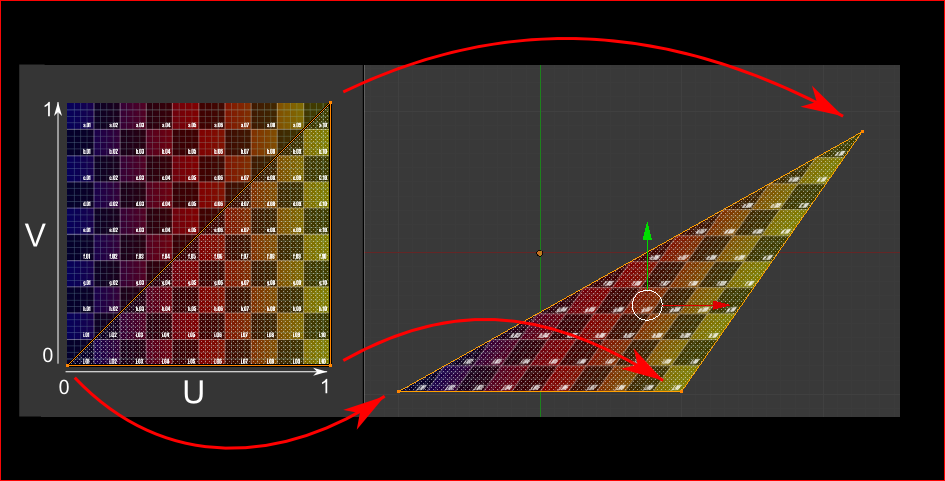
\includegraphics[width=\textwidth]{uv}
	\end{center}
\end{frame}

\fullbleed{character_texture}

\begin{frame}[fragile]{Textures in GLSL}
	Fragment shader:
	
	\begin{lstlisting}[language=GLSL]
in vec2 textureCoords;
uniform sampler2D textureSampler;

void main()
{
    fragmentColour = texture(textureSampler, textureCoords);
}
	\end{lstlisting}
\end{frame}

\begin{frame}[fragile]{Texture filtering}
	\pause
	\begin{lstlisting}
glTexParameteri(GL_TEXTURE_2D, GL_TEXTURE_MIN_FILTER, GL_LINEAR);
glTexParameteri(GL_TEXTURE_2D, GL_TEXTURE_MAG_FILTER, GL_LINEAR);
	\end{lstlisting}
	\begin{itemize}
		\item \textbf{Linear interpolation} (\lstinline{GL_LINEAR})
			smooths between pixels
		\pause\item \textbf{Nearest neighbour} (\lstinline{GL_NEAREST})
			is pixelated but may be slightly faster
		\pause\item \textbf{Anisotropic filtering} improves the quality of linear interpolation
			but is slower
		\pause\item \textbf{Mip-mapping} pre-calculates scaled down versions of the texture ---
			improves quality but costs memory
	\end{itemize}
\end{frame}

\begin{frame}{Texture dimensions}
	\begin{itemize}
		\item In the old days, OpenGL required textures to have \textbf{power of two} dimensions
			\begin{itemize}
				\pause\item $2, 4, 8, 16, 32, 64, 128, 256, 512, 1024, \dots$
			\end{itemize}
		\pause\item Nowadays \textbf{non-power of two (NPOT)} textures are widely supported
		\pause\item Still better to stick to powers of two as some things work better (e.g.\ mipmapping)
		\pause\item NB: \textbf{rectangular} textures are fine, but \textbf{square} textures make UV coordinates saner
	\end{itemize}
\end{frame}

\begin{frame}
	\begin{center}
		Texture Mapping Example
	\end{center}
\end{frame}

\part{Transparency}
\frame{\partpage}

\begin{frame}{Alpha}
	\begin{itemize}
		\pause\item We are used to working with colours in \textbf{RGB} space
		\pause\item We can also work in \textbf{RGBA} space, where A = alpha = transparency
		\pause\item $A=0 \implies$ fully transparent
		\pause\item $A=1$ (or $A=255$) $\implies$ fully opaque
	\end{itemize}
	\pause
	\begin{center}
		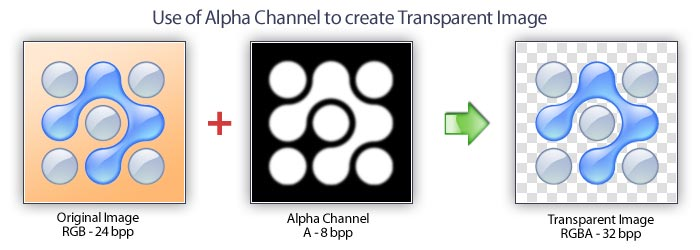
\includegraphics[width=\textwidth]{alpha_channel}
	\end{center}
\end{frame}

\begin{frame}[fragile]{Alpha in OpenGL}
	\begin{itemize}
		\pause\item Use \lstinline[language=GLSL]{vec4} instead of \lstinline[language=GLSL]{vec3} for colours
		\pause\item Textures can have an \textbf{alpha channel}
			\begin{itemize}
				\pause\item PNG supports alpha channels, JPG and BMP do not
			\end{itemize}
		\pause\item Need to enable \textbf{alpha blending}
	\end{itemize}
	\pause
	\begin{lstlisting}
glEnable(GL_BLEND);
glBlendFunc(GL_SRC_ALPHA, GL_ONE_MINUS_SRC_ALPHA);
	\end{lstlisting}
	\begin{itemize}	
		\pause\item Other values can be passed to \lstinline{glBlendFunc} for special effects
			(e.g.\ \textbf{additive blending} is often used for particle effects simulating
				light, fire, explosions etc.)
	\end{itemize}
\end{frame}

\begin{frame}{Transparency and depth testing}
	\begin{itemize}
		\pause\item Recall we are using \textbf{depth testing}
			\begin{itemize}
				\pause\item Each fragment on screen remembers its \textbf{depth} (distance from the camera)
				\pause\item A new fragment is drawn \textbf{only if} its depth value is \textbf{less} than the current depth value
				\pause\item I.e.\ don't draw objects that should be behind something that was already drawn
			\end{itemize}
		\pause\item But if the object in front is (semi-)transparent, we want to see the object behind it!
		\pause\item Solution: draw semi-transparent objects \textbf{after} opaque objects,
			and in \textbf{back to front} order
		\pause\item Further discussion: {\footnotesize\url{http://www.opengl-tutorial.org/intermediate-tutorials/tutorial-10-transparency/}}
	\end{itemize}
\end{frame}

\part{More meshes}
\frame{\partpage}

\begin{frame}{SOH CAH TOA}
	\begin{center}
		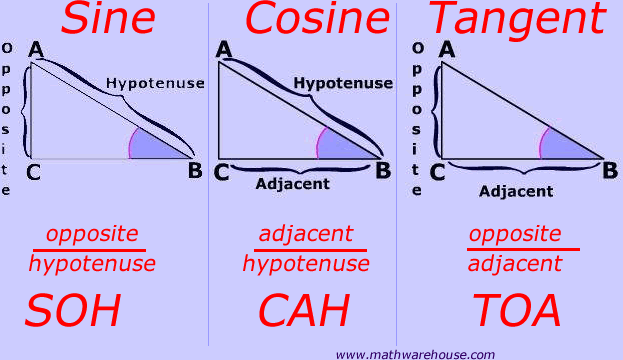
\includegraphics[width=\textwidth]{sohcahtoa}
	\end{center}
\end{frame}

\begin{frame}{Drawing a circle}
	\begin{columns}
		\begin{column}{0.48\textwidth}
			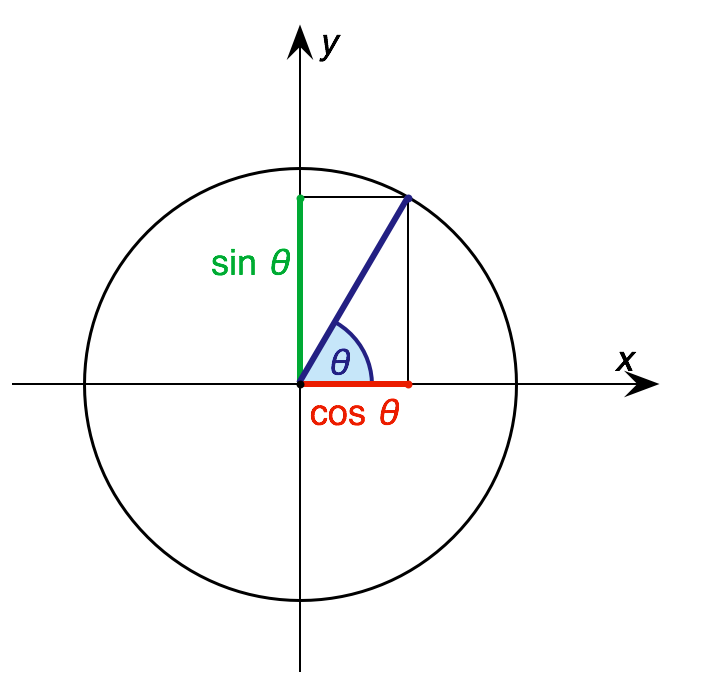
\includegraphics[width=\textwidth]{unit_circle}
		\end{column}
		\begin{column}{0.48\textwidth}
			\pause Circle of \textbf{radius} $r$
			
			\pause $\therefore$ hypotenuse = $r$
			
			\vspace{2ex}
			
			\pause $\cos \theta = \frac{\text{adjacent}}{\text{hypotenuse}} = \frac{x}{r}$
			
			\pause $\therefore x = r \cos \theta$
			
			\vspace{2ex}
			
			\pause $\sin \theta = \frac{\text{opposite}}{\text{hypotenuse}} = \frac{y}{r}$
			
			\pause $\therefore y = r \sin \theta$

			\vspace{2ex}
			
			\pause NB: this works even if $\cos \theta$ and/or $\sin \theta$ are negative
				(i.e.\ if $\theta$ is not between $0^\circ$ and $90^\circ$)
		\end{column}
	\end{columns}
\end{frame}

\begin{frame}{Drawing a cylinder}
	\begin{center}
		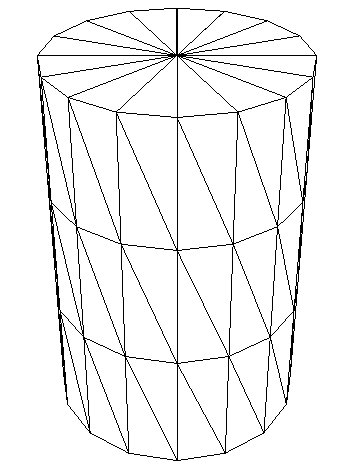
\includegraphics[height=0.8\textheight]{cylinder}
	\end{center}
\end{frame}

\begin{frame}{Drawing a sphere}
	\begin{center}
		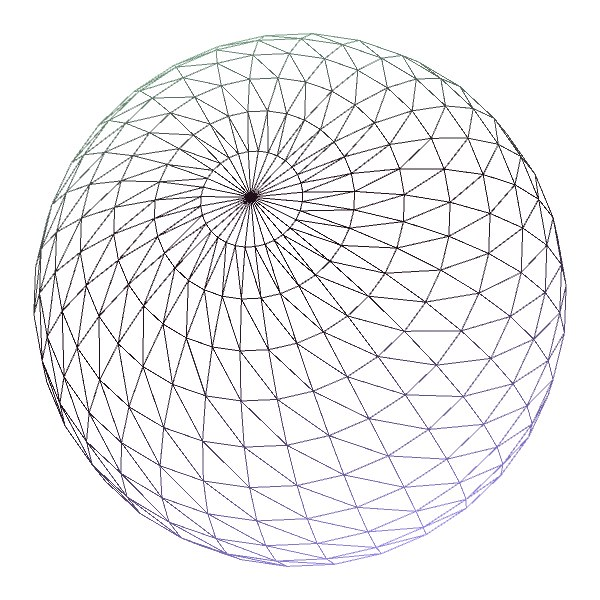
\includegraphics[height=0.8\textheight]{sphere}
	\end{center}
\end{frame}



\begin{frame}{Next steps}
	\begin{itemize}
		\item \textbf{Review} the additional asynchronous material for more background on texture properties and a preview of ways to structure code for importing meshes/models.
		\item \textbf{Attend} the workshop to practice loading textures and meshes from file.
	\end{itemize}
\end{frame}

\end{document}

